\chapter{中断与异常处理}

在操作系统运行中,有三种情况会导致CPU暂停普通指令的执行并强行将控制权转移给处理该事件的特殊代码:
第一种情况是系统调用,用户程序执行ecall指令请求内核为其执行某些操作时;
第二种情况是异常,当指令执行了非法操作时;
第三种情况是设备中断,当设备发出信号提示其需要注意时。
在NimlothOS中,这种情况统称为trap。操作系统对它们通常的处理流程是:

\begin{enumerate}
    \item trap强制将控制权转移到内核
    \item 内核保存寄存器和其他状态以便后续恢复执行
    \item 内核执行适当的处理程序代码
    \item 内核恢复保存的状态并从trap返回
\end{enumerate}

\section{系统设计}

正常情况下陷阱、中断与异常都是由内核的异常处理程序进行处理,它们对用户进程是不可见的,
NimlothOS中,实现了信号机制,使得进程可以得知发生的系统事件。信号机制是一种更高层次的软件形式的异常,
它同样会中断进程的控制流,可以由进程进行处理。因此在本系统中,陷阱处理机制与信号处理机制是紧密结合的。

目前实现的系统处理陷阱类型包括:

\begin{itemize}
    \item \textbf{系统调用}:用户程序通过ecall指令请求内核服务
    \item \textbf{时钟中断}:实现抢占式多进程调度的时间片机制
    \item \textbf{内存访问异常}:数据访问违规、页面错误等内存相关异常
    \item \textbf{指令异常}:非法指令、指令访问错误等执行异常
\end{itemize}

\section{陷阱处理相关硬件}

RISC-V架构为陷阱处理提供了完整的硬件支持,通过一系列控制状态寄存器(CSR)来管理陷阱的触发、处理和恢复过程。
NimlothOS充分利用了这些硬件机制,实现高效的陷阱处理系统。

\subsection{陷阱向量寄存器(stvec)}

\begin{figure}[htbp]
    \centering
    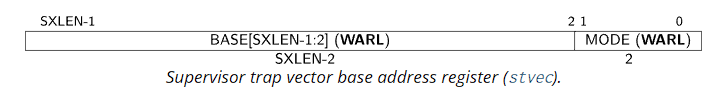
\includegraphics[width=1.0\textwidth]{../image/stvec.png}
    \caption{stvec寄存器}
    \label{fig:stvec}
\end{figure}

\href{https://five-embeddev.com/riscv-priv-isa-manual/Priv-v1.12/supervisor.html#supervisor-trap-vector-base-address-register-stvec}{stvec寄存器}
保存陷阱处理程序的入口地址,是陷阱处理的起始点。当陷阱发生时,硬件会自动将PC设置为stvec中存储的地址,
开始执行陷阱处理代码。

\begin{lstlisting}[language=Rust,caption={陷阱向量寄存器设置}, label={lst:stvec-setup}]
// 设置内核态陷阱入口
fn set_kernel_trap_entry() {
    unsafe {
        stvec::write(trap_from_kernel as usize, TrapMode::Direct);
    }
}
// 设置用户态陷阱入口  
fn set_user_trap_entry() {
    unsafe {
        stvec::write(TRAMPOLINE as usize, TrapMode::Direct);
    }
}
\end{lstlisting}

NimlothOS采用Direct模式,所有陷阱都跳转到同一个入口地址,然后由软件根据陷阱原因进行分发处理。

\subsection{陷阱原因寄存器(scause)}

\begin{figure}[htbp]
    \centering
    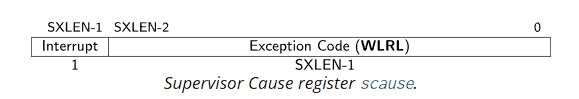
\includegraphics[width=0.8\textwidth]{../image/scause.png}
    \caption{scause寄存器}
    \label{fig:scause}
\end{figure}

\href{https://five-embeddev.com/riscv-priv-isa-manual/Priv-v1.12/supervisor.html#sec:scause}{scause寄存器}
记录了陷阱发生的原因,它的最高位是中断位,用于区分中断和异常,1表示中断,0表示异常,后面则是异常代码,标识具体的异常或中断类型。

scause寄存器的完整编码表如下:

\begin{table}[!htbp]
\centering
\caption{RISC-V陷阱原因编码表}
\label{tab:trap-causes}
\begin{tabular}{|c|c|l|}
\hline
\textbf{中断位} & \textbf{异常代码} & \textbf{描述} \\
\hline
\multicolumn{3}{|c|}{\textbf{中断类型 (Interrupt = 1)}} \\
\hline
1 & 0 & 保留 \\
1 & 1 & 监督者软件中断 \\
1 & 2–4 & 保留 \\
1 & 5 & \textbf{监督者时钟中断} \\
1 & 6–8 & 保留 \\
1 & 9 & 监督者外部中断 \\
1 & 10–15 & 保留 \\
1 & ≥16 & 平台专用 \\
\hline
\multicolumn{3}{|c|}{\textbf{异常类型 (Interrupt = 0)}} \\
\hline
0 & 0 & 指令地址未对齐 \\
0 & 1 & 指令访问错误 \\
0 & 2 & \textbf{非法指令} \\
0 & 3 & 断点 \\
0 & 4 & 加载地址未对齐 \\
0 & 5 & 加载访问错误 \\
0 & 6 & 存储/AMO地址未对齐 \\
0 & 7 & 存储/AMO访问错误 \\
0 & 8 & \textbf{用户态环境调用} \\
0 & 9 & 监督者态环境调用 \\
0 & 10–11 & 保留 \\
0 & 12 & 指令页面错误 \\
0 & 13 & \textbf{加载页面错误} \\
0 & 14 & 保留 \\
0 & 15 & \textbf{存储/AMO页面错误} \\
0 & 16–23 & 保留 \\
0 & 24–31 & 自定义使用 \\
0 & 32–47 & 保留 \\
0 & 48–63 & 自定义使用 \\
0 & ≥64 & 保留 \\
\hline
\end{tabular}
\end{table}

其中,NimlothOS当前处理的关键陷阱类型包括:

\begin{itemize}
    \item \textbf{异常代码5(中断)}:监督者时钟中断,用于实现抢占式调度
    \item \textbf{异常代码8}:用户态环境调用(ecall),对应系统调用
    \item \textbf{异常代码2}:非法指令异常,转换为SIGILL信号
    \item \textbf{异常代码13,15}:加载/存储页面错误,转换为SIGSEGV信号
    \item \textbf{异常代码1,5,7,12}:各种访问错误,转换为SIGSEGV信号
\end{itemize}

\subsection{陷阱值寄存器(stval)}

\begin{figure}[htbp]
    \centering
    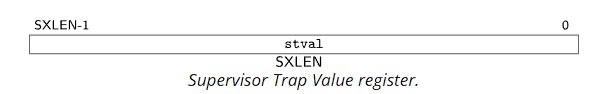
\includegraphics[width=0.7\textwidth]{../image/stval.png}
    \caption{stval寄存器}
    \label{fig:stval}
\end{figure}

\href{https://five-embeddev.com/riscv-priv-isa-manual/Priv-v1.12/supervisor.html#supervisor-trap-value-stval-register}{stval寄存器}提供陷阱相关的辅助信息:

\begin{itemize}
    \item \textbf{地址异常}:存储导致异常的虚拟地址
    \item \textbf{非法指令}:存储非法指令的编码
    \item \textbf{其他异常}:存储相关的错误信息
\end{itemize}

\subsection{监督者状态寄存器(sstatus)}

\begin{figure}[htbp]
    \centering
    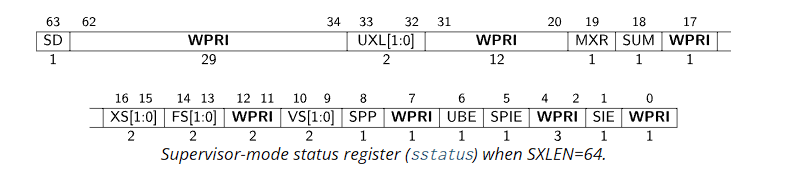
\includegraphics[width=0.8\textwidth]{../image/sstatus.png}
    \caption{sstatus寄存器}
    \label{fig:sstatus}
\end{figure}

\href{https://five-embeddev.com/riscv-priv-isa-manual/Priv-v1.12/supervisor.html#sstatus}{sstatus寄存器}控制处理器的状态和行为,
其中SPP位指示在进入管理模式前执行的特权级别,当发生陷阱时,如果陷阱来自用户态会设置为0,当执行sret指令时,会根据SSP位来恢复特权级别。
SIE位则用于在管理模式下启用或禁用所有中断,当SIE清零时,管理模式下不会接受中断;SPIE位指示在进入管理模式前是否启用了管理中断,当陷阱进入管理模式时,
SPIE位设置成SIE的值,SIE则清零,而执行sret指令时,SIE被设置成SPIE的值,SPIE清零。

\subsection{监督者异常程序计数器(sepc)}

\begin{figure}[htbp]
    \centering
    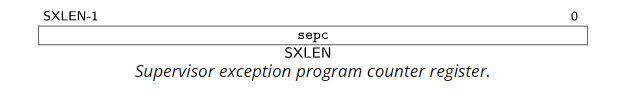
\includegraphics[width=0.7\textwidth]{../image/sepc.png}
    \caption{sepc寄存器}
    \label{fig:sepc}
\end{figure}

\href{https://five-embeddev.com/riscv-priv-isa-manual/Priv-v1.12/supervisor.html#supervisor-exception-program-counter-sepc}{sepc寄存器}
保存触发陷阱的指令地址,当执行sret指令时,sepc的值会被加载到PC寄存器,从而恢复到之前的特权级别。

\subsection{监督者暂存寄存器(sscratch)}

\begin{figure}[htbp]
    \centering
    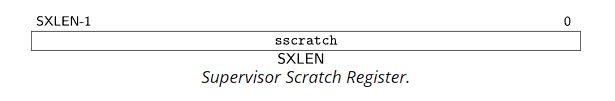
\includegraphics[width=0.7\textwidth]{../image/sscratch.png}
    \caption{sscratch寄存器}
    \label{fig:sscratch}
\end{figure}

\href{https://five-embeddev.com/riscv-priv-isa-manual/Priv-v1.12/supervisor.html#supervisor-scratch-register-sscratch}{sscratch寄存器}
用于在用户态和内核态之间切换时临时存储数据,当用户态执行时,存储陷阱上下文的地址,当陷阱处理时,与sp寄存器交换,实现栈切换。

\subsection{监督者中断使能寄存器(sie)}

\begin{figure}[htbp]
    \centering
    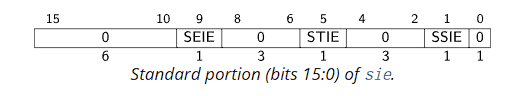
\includegraphics[width=0.7\textwidth]{../image/sie_.png}
    \caption{sie寄存器}
    \label{fig:sie}
\end{figure}

\href{https://five-embeddev.com/riscv-priv-isa-manual/Priv-v1.12/supervisor.html#supervisor-interrupt-registers-sip-and-sie}{sie寄存器}
控制各种中断的使能状态,每一位对应一种中断源:

\begin{itemize}
    \item \textbf{STIE}:时钟中断使能位
    \item \textbf{SEIE}:外部中断使能位  
    \item \textbf{SSIE}:软件中断使能位
\end{itemize}

\begin{lstlisting}[language=Rust,caption={中断使能设置}, label={lst:interrupt-enable}]
pub fn enable_timer_interrupt() {
    unsafe {
        sie::set_stimer(); // 启用时钟中断
    }
}
\end{lstlisting}

\subsection{硬件自动处理}

当陷阱发生时,RISC-V硬件会自动完成以下操作:

\begin{enumerate}
    \item \textbf{保存状态}:将当前特权级和中断状态保存到sstatus
    \item \textbf{记录原因}:将陷阱原因写入scause寄存器
    \item \textbf{保存地址}:将触发陷阱的指令地址保存到sepc
    \item \textbf{记录信息}:将相关信息(如出错地址)保存到stval
    \item \textbf{切换模式}:切换到监督者模式,禁用中断
    \item \textbf{跳转执行}:将PC设置为stvec中的地址开始执行
\end{enumerate}

\subsection{陷阱返回指令(sret)}

sret指令用于从监督者模式返回到之前的特权级,硬件会自动:

\begin{enumerate}
    \item \textbf{恢复PC}:将sepc的值加载到PC寄存器
    \item \textbf{恢复特权级}:根据sstatus.SPP恢复之前的特权级
    \item \textbf{恢复中断}:根据sstatus.SPIE恢复中断使能状态
    \item \textbf{清理状态}:清除sstatus.SPP,将SPIE复制到SIE
\end{enumerate}

\section{陷阱处理机制}

陷阱处理采用硬件与软件协同的方式。当陷阱发生时,RISC-V硬件自动完成特权级切换、
保存关键寄存器状态,然后跳转到内核设置的陷阱向量地址执行。
NimlothOS通过Trampoline页面和陷阱上下文结构,实现了完整的用户态状态保存与恢复机制。

\subsection{Trampoline}

Trampoline是一种地址空间切换机制。由于用户态发生陷阱时仍在用户地址空间中,
直接跳转到内核代码会导致地址转换错误。Trampoline页面同时映射到用户地址空间和内核地址空间的相同虚拟地址,
这样陷阱处理代码在地址空间切换的过程中能够正常找到trap.S放置在trampoline中的切换函数。

\subsection{处理流程}

陷阱处理的完整流程如下:

\begin{enumerate}
    \item \textbf{陷阱触发}:用户程序执行ecall指令或发生异常/中断
    \item \textbf{硬件切换}:CPU自动切换到S模式,跳转到stvec指定的处理程序
    \item \textbf{上下文保存}:\_\_alltraps保存所有寄存器到陷阱上下文
    \item \textbf{地址空间切换}:从用户地址空间切换到内核地址空间
    \item \textbf{处理分发}:trap\_handler根据陷阱类型执行相应处理
    \item \textbf{信号处理}:检查和处理进程待决信号
    \item \textbf{上下文恢复}:\_\_restore恢复寄存器并返回用户态
\end{enumerate}

\begin{figure}[!htbp]
    \centering
    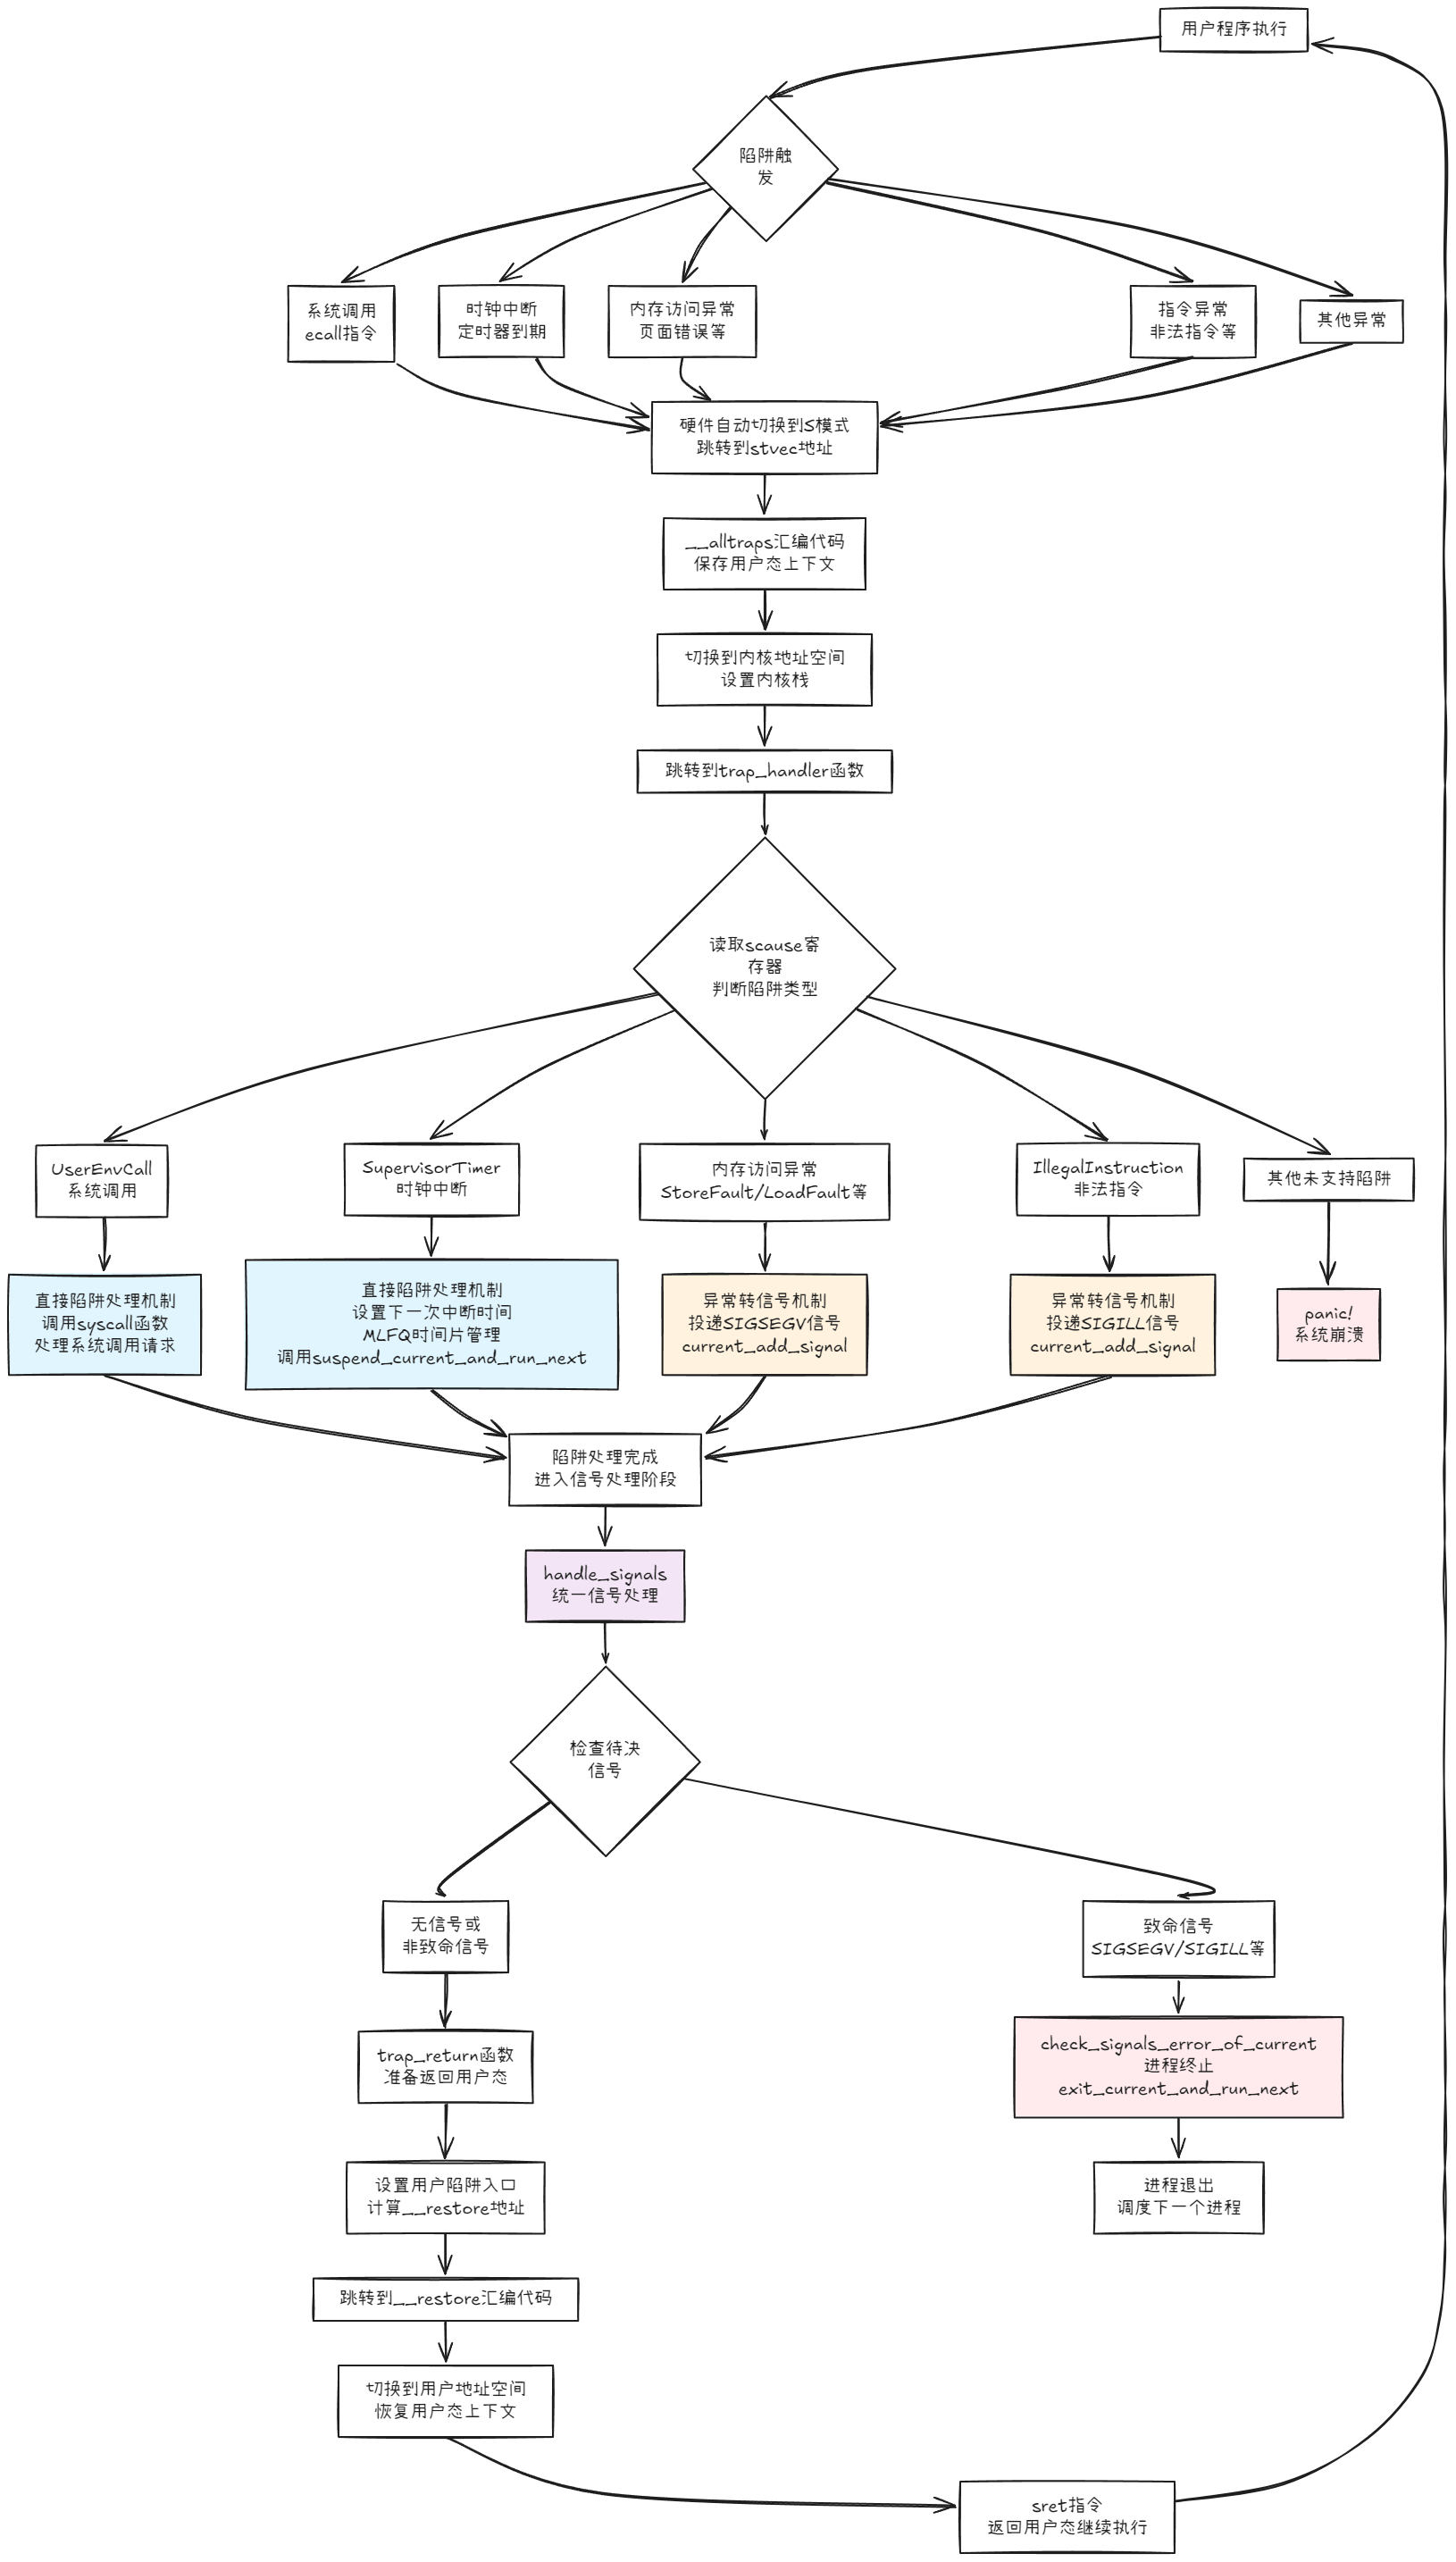
\includegraphics[width=0.8\textwidth]{../image/陷阱信号处理协作.png}
    \caption{陷阱处理流程}
    \label{fig:trap-process}
\end{figure}

\section{时钟中断与抢占调度}

时钟中断是实现抢占式多进程调度的关键机制。系统通过SBI接口设置定时器,
定期触发时钟中断,强制进行进程切换,确保没有进程能够无限期占用CPU资源。

在时钟中断处理中,NimlothOS实现了MLFQ调度算法的时间片管理:
每次中断都会增加当前进程的时间片使用计数,当达到该优先级队列的时间片限制时,
进程会被降级到下一个优先级队列,从而实现动态的优先级调整机制。

\noindent
\rule{0.4\textwidth}{0.4pt}
\hfill
\text{以下为实现介绍}
\hfill
\rule{0.4\textwidth}{0.4pt}

\section{陷阱上下文管理}

陷阱上下文是陷阱处理的核心数据结构,负责保存用户程序触发陷阱时的完整CPU状态。
与进程上下文不同,陷阱上下文需要保存所有寄存器,确保用户程序状态的完整性。

\subsection{陷阱上下文结构}

\begin{lstlisting}[language=Rust,caption={陷阱上下文结构}, label={lst:trap-context}]
#[repr(C)]
#[derive(Clone, Copy, Debug)]
pub struct TrapContext {
    /// 通用寄存器 x0-x31
    pub x: [usize; 32],
    /// 监督者状态寄存器 (sstatus)
    pub sstatus: Sstatus,
    /// 监督者异常程序计数器 (sepc)
    pub sepc: usize,
    /// 内核页表标识符
    pub kernel_satp: usize,
    /// 内核栈指针
    pub kernel_sp: usize,
    /// 陷阱处理函数地址
    pub trap_handler: usize,
}
\end{lstlisting}

陷阱上下文的设计考虑了陷阱处理的完整性和安全性需求。首先是\textbf{完整性保存},
系统保存所有32个通用寄存器,确保用户程序状态不丢失;其次是\textbf{特权级信息},
通过sstatus寄存器记录陷阱前的特权级和中断状态;再次是\textbf{返回地址},
sepc寄存器指向触发陷阱的指令地址,用于陷阱返回时恢复执行;最后是\textbf{内核环境准备},
kernel\_satp、kernel\_sp和trap\_handler三个字段为陷阱处理准备了完整的内核执行环境。

\subsection{上下文初始化}

系统为新创建的用户程序提供初始化陷阱上下文的功能:

\begin{lstlisting}[language=Rust,caption={陷阱上下文初始化}, label={lst:trap-context-init}]
impl TrapContext {
    pub fn app_init_context(
        entry: usize,
        sp: usize,
        kernel_satp: usize,
        kernel_sp: usize,
        trap_handler: usize,
    ) -> Self {
        let mut sstatus = sstatus::read();
        sstatus.set_spp(SPP::User); // 设置返回到用户态
        let mut cx = Self {
            x: [0; 32],
            sstatus,
            sepc: entry, // 设置程序入口地址
            kernel_satp,
            kernel_sp,
            trap_handler,
        };
        cx.sp(sp); // 设置用户栈指针
        cx
    }
}
\end{lstlisting}

初始化过程设置了程序入口地址、用户栈指针、返回特权级等关键信息,
确保用户程序能够在正确的环境中开始执行。

\section{陷阱处理核心}

陷阱处理的核心是trap\_handler函数,它作为所有用户态陷阱的统一入口,
负责分析陷阱类型并执行相应的处理逻辑。

\subsection{陷阱处理主函数}

\begin{lstlisting}[language=Rust,caption={陷阱处理主函数}, label={lst:trap-handler}]
#[unsafe(no_mangle)]
pub fn trap_handler() -> ! {
    set_kernel_trap_entry();
    let scause = scause::read();
    let stval = stval::read();
    match scause.cause() {
        Trap::Exception(Exception::UserEnvCall) => {
            let mut cx = current_trap_cx();
            cx.sepc += 4;
            let result = syscall(cx.x[17], [cx.x[10], cx.x[11], cx.x[12]]);
            cx = current_trap_cx();
            cx.x[10] = result as usize;
        }
        Trap::Exception(Exception::StoreFault)
        | Trap::Exception(Exception::StorePageFault)
        | Trap::Exception(Exception::LoadFault)
        | Trap::Exception(Exception::LoadPageFault)
        | Trap::Exception(Exception::InstructionFault)
        | Trap::Exception(Exception::InstructionPageFault) => {
            current_add_signal(SignalFlags::SIGSEGV);
        }
        Trap::Exception(Exception::IllegalInstruction) => {
            current_add_signal(SignalFlags::SIGILL);
        }
        Trap::Interrupt(Interrupt::SupervisorTimer) => {
            next_trigger();
            // MLFQ 时间片管理逻辑
            suspend_current_and_run_next();
        }
        _ => {
            panic!(
                "Unsupported trap {:?}, stval = {:#x}!",
                scause.cause(),
                stval,
            );
        }
    }

    handle_signals();
    if let Some((errno, msg)) = check_signals_error_of_current() {
        println!("[kernel] {}", msg);
        exit_current_and_run_next(errno);
    }
    trap_return();
}
\end{lstlisting}

\subsection{系统调用处理}

系统调用是用户程序请求内核服务的标准方式。在RISC-V架构中,用户程序通过ecall指令触发系统调用,
系统调用处理涉及多个关键环节。首先是\textbf{参数传递},系统调用号存储在x17寄存器,
而调用参数存储在x10-x12寄存器中;然后是\textbf{返回值处理},系统调用的返回值会写入x10寄存器供用户程序获取;
接下来是\textbf{PC调整},系统需要将sepc增加4来跳过ecall指令,避免陷阱返回后重复执行;
最后是\textbf{上下文管理},由于系统调用处理过程中可能发生进程调度,
因此需要两次获取陷阱上下文来处理可能出现的上下文变化。

\subsection{异常转信号机制}

NimlothOS采用"异常转信号"的方法,将传统的直接杀死进程改为投递信号。
对于\textbf{内存访问异常},系统将其转换为SIGSEGV信号;
对于\textbf{非法指令异常},系统将其转换为SIGILL信号;
这样允许用户程序自定义信号处理函数来应对异常情况;同时达到了\textbf{统一管理}的目标,
通过信号系统统一处理各种异常情况,实现更一致和可控的异常处理机制。

\section{时钟中断与调度}

时钟中断是实现抢占式调度的核心机制,它定期打断用户程序的执行,
给调度器一个重新分配CPU的机会。

\subsection{时钟中断初始化}

系统在启动时需要初始化时钟中断:

\begin{lstlisting}[language=Rust,caption={时钟中断初始化}, label={lst:timer-init}]
pub fn init() {
    set_kernel_trap_entry();
    enable_timer_interrupt();
}
pub fn enable_timer_interrupt() {
    unsafe {
        sie::set_stimer();
    }
}
\end{lstlisting}

\subsection{MLFQ时间片管理}

在时钟中断处理中,系统实现了MLFQ调度算法的时间片管理机制,这个在进程部分已经有过介绍,
这里不再赘述。

\section{底层汇编实现}

陷阱处理的底层切换使用汇编代码,负责寄存器的保存和恢复。

\subsection{陷阱保存机制}

\begin{lstlisting}[language={[x86masm]Assembler},caption={陷阱上下文保存}, label={lst:alltraps}]
__alltraps:
    # 交换 sscratch and sp(x2) 寄存器内容
    csrrw sp, sscratch, sp
    # 现在sp->kernel stack,sscratch->user stack
    # 保存通用寄存器,跳过x0,tp(x4)
    sd x1, 1*8(sp)
    sd x3, 3*8(sp)
    .set n, 5
    .rept 27
        SAVE_GP %n
        .set n, n+1
    .endr
    # 读寄存器并保存
    csrr t0, sstatus
    csrr t1, sepc
    sd t0, 32*8(sp)
    sd t1, 33*8(sp)
    # sscratch 现在指向用户栈
    csrr t2, sscratch
    sd t2, 2*8(sp)
    # 保存kernel_satp到t0
    ld t0, 34*8(sp)
    # 保存trap_handler到t1
    ld t1, 36*8(sp)
    # 跳转到kernel_sp
    ld sp, 35*8(sp)
    # 切换到内核地址空间
    csrw satp, t0
    sfence.vma
    # 跳转到trap_handler
    jr t1
\end{lstlisting}

保存过程按照严格的顺序执行五个关键步骤。首先进行\textbf{栈指针切换},
通过sscratch寄存器实现用户栈到内核栈的切换;接着进行\textbf{寄存器保存},
逐个保存所有通用寄存器到陷阱上下文中确保状态完整性;然后是\textbf{CSR保存},
保存sstatus和sepc等关键控制寄存器的状态信息;随后执行\textbf{地址空间切换},
更新satp寄存器将执行环境从用户地址空间切换到内核地址空间;
最后\textbf{跳转执行},跳转到trap\_handler函数开始内核态的陷阱处理流程。

\subsection{陷阱恢复机制}

\begin{lstlisting}[language={[x86masm]Assembler},caption={陷阱上下文恢复}, label={lst:restore}]
__restore:
    # 切换到用户地址空间
    csrw satp, a1
    sfence.vma
    csrw sscratch, a0
    mv sp, a0
    # 恢复CSR和通用寄存器
    ld t0, 32*8(sp)
    ld t1, 33*8(sp)
    csrw sstatus, t0
    csrw sepc, t1
    ld x1, 1*8(sp)
    ld x3, 3*8(sp)
    .set n, 5
    .rept 27
        LOAD_GP %n
        .set n, n+1
    .endr
    # 恢复用户栈指针
    ld sp, 2*8(sp)
    sret
\end{lstlisting}

恢复过程与保存过程相反,按照逆序执行五个步骤来完整恢复用户态执行环境。
首先进行\textbf{地址空间切换},将执行环境从内核地址空间切换回用户地址空间;
接着进行\textbf{CSR恢复},恢复sstatus和sepc等关键控制寄存器的状态;
然后执行\textbf{寄存器恢复},逐个恢复所有通用寄存器到用户程序被中断前的状态;
随后进行\textbf{栈指针恢复},将栈指针切换回用户程序的栈;
最后执行\textbf{返回用户态},通过sret指令完成特权级切换并跳转回用户程序继续执行。

\section{陷阱返回机制}

陷阱处理完成后,系统需要通过trap\_return函数安全地返回用户态。

\subsection{返回流程}

\begin{lstlisting}[language=Rust,caption={陷阱返回实现}, label={lst:trap-return}]
#[unsafe(no_mangle)]
pub fn trap_return() -> ! {
    set_user_trap_entry();
    let trap_cx_ptr = TRAP_CONTEXT;
    let user_satp = current_user_token();
    unsafe extern "C" {
        fn __alltraps();
        fn __restore();
    }
    let restore_va = __restore as usize - __alltraps as usize + TRAMPOLINE;
    unsafe {
        asm!(
            "fence.i",
            "jr {restore_va}",
            restore_va = in(reg) restore_va,
            in("a0") trap_cx_ptr,
            in("a1") user_satp,
            options(noreturn),
        );
    }
}
\end{lstlisting}

返回过程首先进行\textbf{用户陷阱入口设置},重新配置stvec寄存器指向Trampoline页面,
为后续可能的陷阱做好准备;接着\textbf{准备参数},将陷阱上下文地址和用户页表标识符
作为参数传递给恢复函数;然后执行\textbf{地址计算},计算\_\_restore函数在Trampoline中的正确虚拟地址;
最后进行\textbf{跳转恢复},通过内联汇编跳转到\_\_restore函数开始执行恢复过程。

\section{信号处理集成}

陷阱处理系统与信号处理机制紧密集成,每次陷阱处理完成后都会检查进程的待决信号:

\begin{lstlisting}[language=Rust,caption={信号处理集成}, label={lst:signal-integration}]
handle_signals();

if let Some((errno, msg)) = check_signals_error_of_current() {
    println!("[kernel] {}", msg);
    exit_current_and_run_next(errno);
}

trap_return();
\end{lstlisting}
